\documentclass[12pt,notitlepage,nofootinbib]{revtex4}
\usepackage{graphicx}
\usepackage{bm}
\usepackage{rotating}
\def\baselinestretch{1.2}
\usepackage{dcolumn}
\usepackage{times}
\usepackage{color}
\usepackage{amsmath} 
\usepackage{extarrows}
\usepackage{listings}
\usepackage{url}
\setlength{\mathindent}{0pt}

\begin{document}

\title{StochSS Hands-on Tutorial Series: 3 - Population Dynamics with StochSS}

\author{StochSS Development Team}
\affiliation{Department of Computer Science - University of California, Santa Barbara}

\date{\today}

\maketitle

\section{\label{sec:pre}Prerequisites}
\begin{itemize}
\item StochSS 1.2 (or later) installed on your computer (please follow download and installation instructions at \url{www.stochss.org}). 
\item A basic understanding of well mixed discrete stochastic simulations and models based on ordinary differential equations. 
\item The following login screen appears on your browser: please log in.
\end{itemize}

\begin{figure}[!htb]
\centering
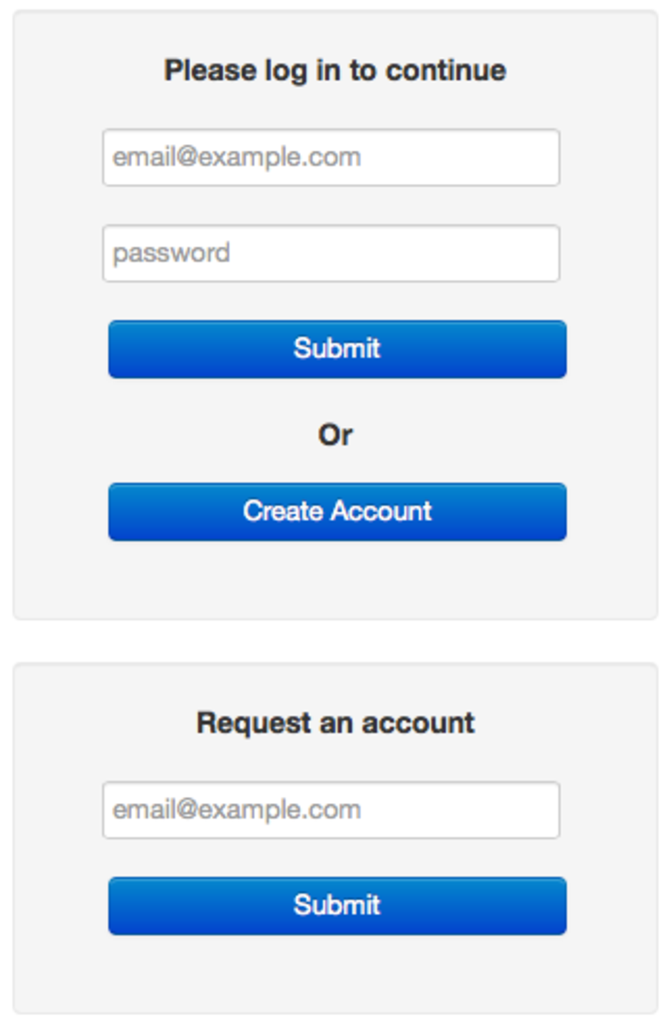
\includegraphics[scale=0.64]{user-login.pdf}
\end{figure}

\section{The Lotka-Volterra equations}

chemistry and ecology all together ...

\subsection{Refinements}

\subsubsection{Prey logistic growth}

\subsubsection{Predator type II functional response}

\section{A Genetic Toggle Switch}

\newpage

\begin{thebibliography}{9}

\bibitem{lotka}
  A.J. Lotka ,
  \textit{Contribution to the theory of periodic reactions}.
  J. Phys. Chem., 14 (3), 271�274 (1910)
  
  \bibitem{volterra}
  V. Volterra,
  \textit{Fluctuations in the abundance of a species considered mathematically}.
  Nature, 118(2972), 558-560 (1926)
  
  \bibitem{gtswitch}
  T.S. Gardner, C.R. Cantor and J.J. Collins
  \textit{Construction of a genetic toggle switch in Escherichia coli}. 
  Nature, 403, 339-342 (2000)
  
\end{thebibliography}

\end{document}
